\section{Implementierung}
\label{sec:implementation}
\subsection{Modellwahl}
\label{ssec:modelwahl}
Wie in Abschnitt \ref{ssec:modellselektion} beschrieben, benötigen wir zur Auswahl der relevanten Prädiktoren die erste Ableitung der Reflektionswerte. Die Methode \textit{getSlope} berechnet diese als Differenz benachbarter Messwerte. Daraus ergibt sich in Methode \textit{criterionSlopeDist} die Variabilität je Wellenlänge als Differenz des größten und des kleinsten Wertes. Alle Wellenlängen mit einer Variablität größer einem vorgegebenen Schwellwert (hier: $0.001$) werden in Methode \textit{selectFeatures} für das Maximalmodell ausgewählt. Alle ausgewählen Variablen gehen linear in das Maximalmodell ein.\\
Mittels der im Paket \text{leaps} bereitgestellten Methode \text{regsubsets} wird aus dem 149 Prädiktoren umfassenden Maximalmodell das Modell als Bestes bestimmt, welches den kleinsten $C_p$ Wert aufweist. Die Variablen sowie die geschätzen Parameter des ausgewählen Modells sind in Tabelle \ref{table:model_parameters} dargestellt.\\
\begin{figure*}[ht]
    \centering
    \begin{tikzpicture}
        \begin{axis}[ 
            ylabel = $var(\delta(\lambda))$,
            xlabel = $\lambda$,
            xmin=1400, xmax=2700,
            ymin=0, %ymax=800,
            legend pos = north west,
            scaled ticks = false,
            width = \textwidth,
            height = 8cm,
            ymajorgrids,
            xmajorgrids,
            cycle list name=auto
        ]
            \addplot +[stack plots=y, no marks, thick]
            table[x=x,y=y,col sep=comma] {plots/data/slopeValues.csv};
            \addlegendentry{{\scriptsize Variablität}}
            
            \addplot +[ycomb, no marks, dashed] 
            table[x=x, y expr=0.0105 ,col sep=comma] {plots/data/selectedFeatures.csv};
            
            \begin{scope}[]
                \draw[] ({rel axis cs:1,0}|-{axis cs:0,0.001}) -- ({rel axis cs:0,0}|-{axis cs:0,0.001});
            \end{scope}
        \end{axis}
    \end{tikzpicture}
    \captionof{figure}{Variablität der Reflektionswerte. Die horizontale Linie markiert den Schwellwert von 0.001, die vertikalen Linien die im optimalen Modell enthaltenen Features. }
    \label{fig:selected_feat}
\end{figure*}


\subsection{Simulation}
Das so ausgewählte, optimale Modell wird nun verwendet, um Pseudobeobachtungswerte zu simulieren. Die Simulation erfolgt in mehreren Runden und für verschiedene Stichprobengrößen von 150, 200, 250, 300, 350, 400, 450 und 500 zufällig ausgewählten sowie für die gesamten 533 Spektren des vorliegenden Datensatzes. In Methode \textit{simulateOnDatSubset} erfolgt zunächst die zufällige Auswahl der übergebenen Anzahl an Sprektren. Anschließend wird das unter Abschnitt \ref{ssec:modelwahl} bestimmte, optimale Modell verwendet, um neue Stockstoffwerte zu erzeugen, wobei, wie in Abschnitt \ref{ssec:Theoretische Grundlagen der Simulation} beschrieben, eine Normalverteilung der Zufallsgröße angenommen wird. In jedem Simulationsdurchlauf wird der Ergebnisvektor als arithmetisches Mittel aus 1000 Durchgängen erzeugt. \\
Mit den so erzeugten Pseudobeobachtungen, sowie den originalen Reflektionswerten wird nun ein zweites mal die Methode \textit{regsubsets} aus dem \textit{leaps} Paket aufgerufen, um für den neuen Datensatz das beste Modell mittels Mallows' $C_p$-Kriterium zu bestimmen. Für jedes beste Modell wird die Modellgröße sowie der $C_p$-Wert erfasst.\\
Im Anschluss an die Somulation erfolgt die Berechnung des erwarteten Prognosefehler, welche in Methode \textit{calculateTrueSpse} nach Formel (\ref{eq:spse_true}) erfolgt. Die Schätzung des erwarteten Prognosefehlers aus den CP Werten der Simulation erfolgt in Methode \textit{calculateEstimatedSpse} nach der Formel
\[
\hat{\m{SPSE}}^{\m{(M)}} \define (C_p^{\m{(M)}} + (|M| + 1)) \Tilde{\sigma}^2_{full}
\]

\begin{figure*}[ht]
    \centering
    \begin{tikzpicture}
        \begin{axis}[ 
            ylabel = $N_{origin}$,
            xlabel = $N_{est}$,
            xmin=0, xmax=0.8,
            ymin=0, ymax=0.8,
            legend pos = north west,
            scaled ticks = false,
            width = .5\textwidth,
            ymajorgrids,
            xmajorgrids,
            %height = 8cm,
            cycle list name=black white
        ]
            \addplot +[only marks]
            table[x=origN, y=simN, col sep=comma] {plots/data/correlation_plot_data.csv};
            %\addlegendentry{{\scriptsize Variablität}}
            \begin{scope}[red]
                \draw[red] ({axis cs:0,0}) -- ({axis cs:1,1});
            \end{scope}   
            %\addplot +[ycomb, no marks, dashed] 
            %table[x=x, y expr=0.0105 ,col sep=comma] {plots/data/selectedFeatures.csv};
            
            
        \end{axis}
    \end{tikzpicture}
    \captionof{figure}{Korrelationsplot}
    \label{fig:correlation}
\end{figure*}
\begin{figure*}[ht]
    \centering
    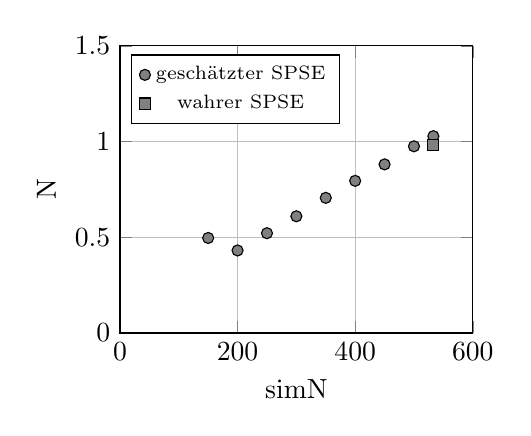
\begin{tikzpicture}
        \begin{axis}[ 
            ylabel = N,
            xlabel = simN,
            xmin=0, xmax=600,
            ymin=0, ymax=1.5,
            legend pos = north west,
            scaled ticks = false,
            width = .5\textwidth,
            ymajorgrids,
            xmajorgrids,
            %height = 8cm,
            cycle list name=black white
        ]
            \addplot +[only marks]
            coordinates {
                (150,0.4964226)
                (200,0.4312206)
                (250,0.5213190)
                (300,0.6097658)
                (350,0.7058959)
                (400,0.7947748)
                (450,0.8807918)
                (500,0.9750933)
                (533,1.0280917)
            };
            \addlegendentry{{\scriptsize geschätzter SPSE}}
            
            \addplot +[only marks]
            coordinates {
                (533,0.9813258)
            };
            \addlegendentry{{\scriptsize wahrer SPSE}}
            
            %\addplot +[ycomb, no marks, dashed] 
            %table[x=x, y expr=0.0105 ,col sep=comma] {plots/data/selectedFeatures.csv};
        \end{axis}
    \end{tikzpicture}
    \captionof{figure}{SPSE}
    \label{fig:spse}
\end{figure*}
		
% section implementation